\documentclass[12pt, a4paper]{article}

\usepackage[utf8]{inputenc}
\usepackage[T2A]{fontenc}
\usepackage[russian]{babel}
\usepackage[]{float}

\usepackage[oglav, boldsect, eqwhole, figwhole, %
   remarks, hyperref, hyperprint]{fn2kursstyle}

\frenchspacing
\righthyphenmin=2

%Командна для римских прописных 
\newcommand{\RomanNumeralCaps}[1]
    {\MakeUppercase{\romannumeral #1}}

\title{Итерационные методы решения систем линейных алгебраических уравнений}
\group{ФН2-52Б}
\author{A.\,И.~Токарев}
\secauthor{Ю.\,А.~Сафронов}
\supervisor{}
\date{2021}

\def\hmath$#1${\texorpdfstring{{\rmfamily\textit{#1}}}{#1}}

\begin{document}
\maketitle
\tableofcontents 
\newpage

\section{Краткое описание алгоритмов}
Дана система линейных алгебраических уравнений:
\begin{equation}
\sum_{j=1}^{n} a_{ij}x_i = f_i , \quad i = \overline{1,n}.
\label{Sys}
\end{equation}

Будем искать решение итерационными методами, т.е. последовательно приближаясь к решению. Общий вид стационарных итерационных методов:

\[
B\dfrac{x^{k+1}-x^k}{\tau} + Ax^k = f.
\]

\subsection{Метод простой итерации}

\[
B = E, \quad \dfrac{x^{k+1}-x^k}{\tau} + Ax^k = f, \quad k \in \mathbb{N};
\]
\[
x^k = -(\tau A - E)x^{k-1} + \tau f.
\]

\subsection{Метод Якоби}
Представим матрицу $A$ в виде суммы
\[
A = L + D + U,
\]
где $L$ --- нижняя треугольная, $U$ --- верхняя треугольная, а $D$ - диагональная матрицы.

\[
B = D, \quad D(x^{k-1}-x^k) +  Ax^k = f, \quad k \in \mathbb{N}; 
\]
\[
 x^{k+1} = -D^{-1}(L + U)x^k + D^{-1}f.
\]

\subsection{Методы релаксации и Зейделя}

\[
B = D + \omega L, \quad \tau = \omega \quad (D + \omega L)\dfrac{x^{k+1} - x^k}{\omega} + Ax^k = f, \quad k \in \mathbb{N};
\]
\[
(E + \omega D^{-1}L)x^{k+1} = ((1 - \omega)E - \omega D^{-1}U)x^k + \omega D^{-1}f;
\]

$\omega > 0$ --- метод релаксации, $\omega = 1$ --- частный случай, метод Зейделя.

Для метода релаксации существуют удобные расчетные формулы, которые помогают упростить вычисления. 

\[
x_{i}^{k+1} + \omega\sum_{j = 1}^{i - 1}\dfrac{a_{ij}}{a_{ii}}x_{j}^{k+1} = (1 - \omega)x_i^k - \omega\sum_{j = i + 1}^{n}\dfrac{a_{ij}}{a_{ii}}x_j^k + \omega\dfrac{f_i}{a_{ii}}, i=\overline{1,..., n} ;
\]
\[
x_1^{k+1} = (1 - \omega)x_1^k - \omega\sum_{j = 2}^{n}\dfrac{a_{1j}}{a_{11}}x_j^k + \omega \dfrac{f_1}{a_{11}};
\]

\[
x_2^{k+1} = -\omega\dfrac{a_{21}}{a_{22}}x_1^{k+1} +(1 - \omega)x_2^k - \omega\sum_{j = 3}^{n}\dfrac{a_{2j}}{a_{22}}x_j^k + \omega \dfrac{f_2}{a_{22}};
\]

\centerline{...}

\[
x_i^{k+1} = -\omega\sum_{j=1}^{i-1}\dfrac{a_{ij}}{a_{ii}}x_j^{k+1} +(1 - \omega)x_i^k - \omega\sum_{j = i+1}^{n}\dfrac{a_{ij}}{a_{ii}}x_j^k + \omega \dfrac{f_i}{a_{ii}}, \quad i = \overline{3,4,..., n-1};
\]

\[
x_n^{k+1} = -\omega\sum_{j=1}^{i-1}\dfrac{a_{nj}}{a_{nn}}x_j^{k+1} +(1 - \omega)x_n^k  + \omega \dfrac{f_n}{a_{nn}}
\]




\section{Исходные данные}
Для СЛАУ матрица $A$ и столбец правой части $f_A$ имеют вид 

\[
    A = 
    \begin{pmatrix}
     175.4000    &     0.0000   &      9.3500    &    -0.960\\
  0.5300  &     -46.0000   &      0.2300    &     5.1900\\
 -0.6300    &     5.4400  &     190.6000     &    9.7000\\
  6.2300     &   -8.8900     &   -9.8800    &  -153.4000
  

    \end{pmatrix}, \quad f_{A} = 
    \begin{pmatrix}
 985.3600\\
 348.170\\
2284.7700\\
-638.7800\\

    \end{pmatrix}.
\]

Так же нужно решить СЛАУ с трехдиагональной матрицей $A$ размерности $n = 220$. 

\[
   \begin{pmatrix}
     b_1   &     c_1   &      0    &    ... & 0\\
     a_2 &     b_2   &      c_2    &   ... & 0\\
     0   &    a_3  &     b_3     &   ... & 0 \\
     ...   &    ...  &    ...     &   ... & ...\\ 
     0 & ...    &   a_{n-1}    &   b_{n-1}   &  c_{n-1} \\
     0 & ... & 0 & a_n & b_n\\
    \end{pmatrix} \cdot
    \begin{pmatrix}
 x_1\\
 x_2\\
x_3\\
...\\
x_{n-1}\\
x_n
    \end{pmatrix} =
\begin{pmatrix}
 f_1\\
 f_2\\
f_3\\
...\\
f_{n-1}\\
f_n
    \end{pmatrix},
\]
$a_i = c_i = 1; b_i = 4; i=\overline{1,...,n}; d_1 = 6; d_i = 10 - 2(i \mod 2), i = \overline{2,..., n-1}; d_n = 9 - 3(n \mod 2).$
\newpage

\section{Результаты расчетов}
Результаты с точностью $\varepsilon = 10^{-7}$ приведены в таблице.
\noindent\begin{center}
\hspace*{-25mm}\begin{tabular}{|c|c|c|c|c|c|c|c|c|}
\hline
Метод & $||C||$  & Оценка  & Крит. 1.  & Крит. 1. & Крит. 2.  &Крит. 2. & Крит. 3.& Крит. 3.  \\
&$||G_1||$ & числа &Норма&  Число  & Норма & Число &  Норма& Число  \\
& $||G_2||$ &итераций & ошибки &  итераций & ошибки & итераций &ошибки & итераций \\
\hline
П. И. &&&&&&&& \\
$\tau =0{.}0089$ &$0{.}8367$&104&$5{.}927\cdot 10^{-9}$&62&$5{.}384\cdot10^{-7}$&49&$3{.}357\cdot10^{-8}$&57 \\
\hline
П. И. &&&&&&&&\\
$\tau =0{.}007$ &$0{.}7196$&54&$2{.}588\cdot10^{-6}$&38&$2{.}588\cdot10^{-6}$&38&$1{.}653\cdot10^{-7}$&45 \\
\hline
Якоби &$0{.}1630$&9&$1{.}906\cdot10^{-8}$&8&&&& \\
\hline
Зейдель&$0{.}3115$&8&$1{.}181$&2&&&& \\
&$0{.}1033$&&&&&&& \\
\hline
Релакс &$0{.}4050$&57&$1{.}181$&19&&&& \\
$\omega =1.3$ &$0{.}4343$&&&&&&& \\
\hline
Релакс &$0{.}0935$&85&$1{.}181$&56&&&& \\
$\omega =0.3$ &$0{.}731$&&&&&&& \\
\hline
\end{tabular}
\end{center}
\newpage

\section{Контрольные вопросы}
\begin{enumerate}
\item Почему условие $\|C\| < 1$ гарантирует сходимость итерационных методов решения СЛАУ?
 
$\|x^{k+1}-x^{k}\|=\|(Cx^{k}+y)-(Cx^{k-1}+y)\|=\|C(x^{k}-x^{k-1})\| \leq \|C\| \|x^{k}-x^{k-1}\|$
Пусть $\|C\| < 1$, следовательно, оператор $C$ является сжимающим. 
Существует единственная неподвижная точка $x$, которая и является решением системы. 

Пусть $x^{*}$ $-$ решение СЛАУ $Ax=b$, которое которое мы решаем итерационным методом $x^{k+1}=Cx^{k}+y$, тогда:\\
$$x^{k+1}-x^{*}=(Cx^{k}+y)-(Cx^{*}+y)=C(x^{k}-x^{*}),$$
тогда, если $\|C\| < 1$, то\\
 $\|x^{k+1}-x^{*}\| = \|C(x^{k}-x^{*})\| \leq \|C\|\|x^{k}-x^{*}\| \leq \|C\|^{2} \|x^{k-1}-x^{*}\| \leq \ldots \leq $\\
$\leq \|C\|^{k+1}\|x^{0}-x^{*}\| \rightarrow 0$ при $ k \to \infty$
\\

\item Каким следует выбирать итерационный параметр $\tau$ в методе простой итерации для увеличения скорости сходимости? Как выбрать начальное приближение $x^{0}$?

Нужно выбрать значение $\tau \in (0; \dfrac{2}{\lambda_{max}})$, чтобы норма матрицы $C$ была минимальной. Оптимальным будет значение $\tau = \dfrac{2}{\lambda_{min} + \lambda_{max}}$. Начальное приближение можно выбрать любым.

\item На примере системы из двух уравнений с двумя неизвестными дайте геометрическую интерпретацию метода Якоби, метода Зейделя и метода релаксации.

 \textbf{Геометрическая интерпретация метода Зейделя.}\\
Приведём геометрическую интерпретацию метода Зейделя в случае $m=2$, т.е. в случае решения системы:\\
 \begin{equation*}
 \begin{cases}
  a_{11}x_{1}+a_{12}x_{2}=b_{1},\\
  a_{21}x_{1}+a_{22}x_{2}=b_{2}.
 \end{cases}
\end{equation*}

Первое уравнение системы задаёт на плоскости $x_{1}Ox_{2}$ прямую $l_{1}$, второе - прямую $l_{2}$ (рис. \eqref{figzend}). Расчётные формулы метода принимают следующий вид:

\begin{equation*}
\begin{cases}
x_{1}^{(k+1)}=b_{12}x_{2}^{(k)}+c_{1},\\
x_{2}^{(k+1)}=b_{21}x_{1}^{(k)}+c_{2},\\
\end{cases}
\end{equation*}
где $b_{12}=-\frac{a_{12}}{a_{11}},~ c_{1}=\frac{b_{1}}{a_{11}},~ b_{21}=-\frac{a_{21}}{a_{22}},~ c_{2}=\frac{b_{2}}{a_{22}}.$
\begin{figure}[h]
\center{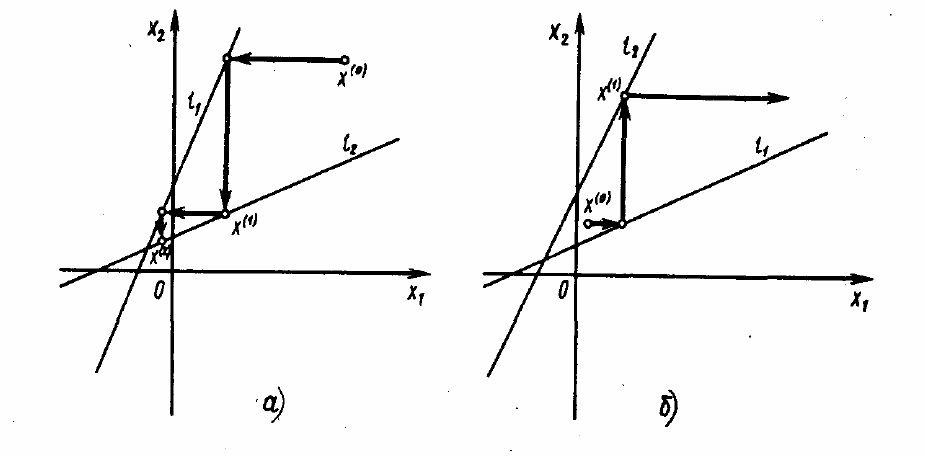
\includegraphics[width=\linewidth]{pic/Зейдель.png}}
\caption{Графическая интерпретация метода Зейделя.}
\label{figzend}
\end{figure}

Пусть приближение $x^{(k)}$ уже найдено. Тогда при определении $x_{1}^{(k+1)}$ координата $x_{2}=x_{2}^{(k)}$ фиксируется и точка $x$ перемещается параллельно оси $Ox_{1}$ до пересечения с прямой $l_{1}$.

Координата $x_{1}$ точки пересечения принимается за $x_{1}^{(k+1)}$. Затем точка $x$ перемещается вдоль прямой $x_{1}=x_{1}^{(k+1)}$ до пересечения с прямой $l_{2}$. Координата $x_{2}$ точки пересечения принимается за $x_{2}^{(k+1)}$.

На рис. \eqref {figzend} приведены геометрические иллюстрации, отвечающие сходящемуся и расходящемуся итерационному процессу Зейделя. Видно, что характер сходимости может измениться при перестановке уравнений.

\textbf{Метод релаксации.}

Суть метода релаксации состоит в том, что после вычисления очередной $i$-ой компоненты $(k+1)$-го приближения по формуле Зейделя

\[
\widetilde x_{i}^{(k+1)}=b_{i1}x_{1}^{(k+1)}+b_{i2}x_{2}^{(k+1)}+ \ldots + b_{i,i-1}x_{i-1}^{(k+1)}+ b_{i,i+1}x_{i+1}^{(k)} + \ldots + b_{im}x_{m}^{(k)}+c_{i} \]

производят дополнительно смещение этой компоненты на величину $(\omega -1)(\widetilde x_{i}^{(k+1)}-x_{i}^{(k)})$, где $\omega$-параметр релаксации. Таким образом, $i$-ая компонента $(k+1)$-го приближения вычисляется по формуле:

\[
x_{i}^{(k+1)}=\widetilde x_{i}^{(k+1)}+(\omega -1)(\widetilde x_{i}^{(k+1)} -x_{i}^{(k)})=\omega\widetilde x_{i}^{(k+1)} + (1-\omega)x_{i}^{(k)}.
\]

На рис.\eqref{fig:picture} показано несколько первых итераций метода при значении параметра релаксации $\omega=1.25$.\\
	
\begin{figure}[H]
\center{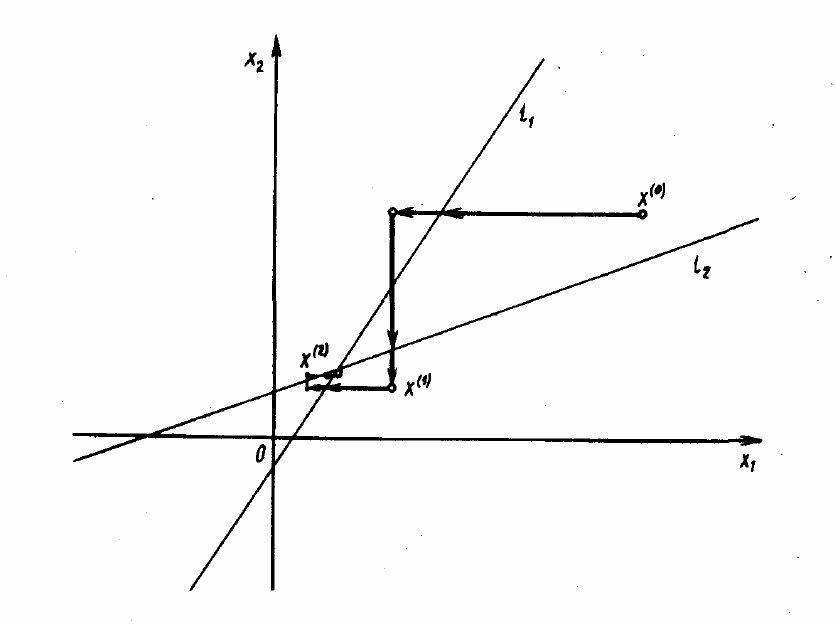
\includegraphics[scale=0.85]{pic/релакс.png}}
\caption{Графическая интерпретация метода релаксации.}
\label{fig:picture}
\end{figure}
	
	
При $\omega = 1$ метод релаксации совпадает с методом Зейделя. При $\omega > 1$ его называют методом последовательной верхней релаксации, а при $\omega < 1$ - методом последовательной нижней релаксации. \\
	
\begin{figure}[H]
\center{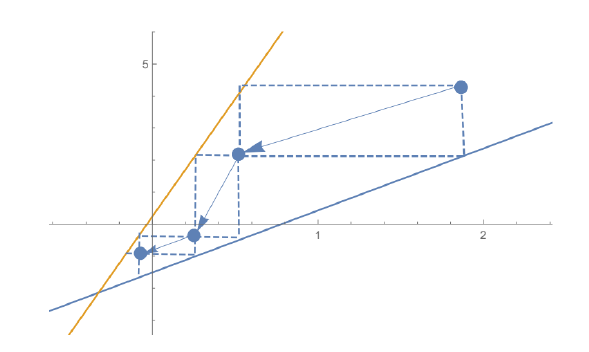
\includegraphics[scale=0.85]{pic/Якоби.png}}
\caption{Графическая интерпретация метода Якоби.}
\label{fig:yakobi}
\end{figure}
	
Если домножить одно из уравнений на $(-1)$, то изменится только направление движения по $x_{i}$ (но не величина, с которой двигаемся). 

Если поменять порядок уравнений местами, то прямые, задаваемые данными уравнениями, поменяются местами. В обоих случаях гарантировать сходимость/расходимость невозможно.
	

	
\item При каких условиях сходятся метод простой итерации, метод Якоби, метод Зейделя и метод релаксации? Какую матрицу называют положительно определённой?

\textbf{Сходимость метода простой итерации.}\\
Пусть выполнено условие 
$$\|B\|<1.$$

Тогда: 1) решение $\overline x$ системы $x=Bx+c,$ где $B$ --- квадратная матрица с элементами $b_{ij} (i,j=1,2,\ldots,m), c$ --- вектор-столбец с элементами $c_{i} (i=1,2,\ldots,m),$ существует и единственно;

2) при произвольном начальном приближении $x^{0}$ метод простой итерации сходится и справедлива оценка погрешности: 
$$ \|x^{(n)}-\overline x\| \leq \|B\|^{n}\|x^{(0)}-\overline x\|.$$
		
\textbf{Сходимость метода Зейделя.}\\
\textbf{Теорема:}
Пусть $\|B\|<1$, где $\|B\|$ - одна из норм $\|B\|_{\infty},\|B\|_{1}.$ Тогда при любом выборе начального приближения $x^{0}$ метод Зейделя сходится со скоростью геометрической прогрессии, знаменатель которой $q \leq \|B\|$.

\textbf{Теорема:}
Пусть выполнено условие $\|B_{1}\|+\|B_{2}\| < 1.$ Тогда при любом выборе начального приближения метод Зейделя сходится и верна оценка погрешности:
$$ \|x^{(n)}-\overline x\| \leq q^{n}\|x^{(0)}-\overline x\|,$$
где $q=\frac{\|B_{2}\|}{(1-\|B_{1}\|)}<1.$ 

\textbf{Теорема:}
Пусть $A$-симметричная положительно определённая матрица. Тогда при любом выборе начального приближения $x^{(0)}$ метод Зейделя сходится со скоростью геометрической прогрессии.

\textbf{Сходимость метода релаксации.}

Если $A$ --- симметричная положительно определённая матрица, то при любом значении параметра $\omega$ $(0<\omega<2)$ метод релаксации сходится. Можно выбрать параметр $\omega>1$ так, чтобы метод релаксации сходился существенно быстрее, чем методы Якоби и Зейделя. 
	
\textbf{Сходимость метода Якоби.}
Пусть $A$ --- симметричная положительно определённая матрица с диагональным преобладанием, т.е. $a_{ii} > \sum\limits_{i \neq j}|a_{ij}|, i=1,2,\ldots,n.$ Тогда метод Якоби сходится. 
		
Матрица $A$  называется положительно определённой, если $\exists \delta>0: (Ax,x) \geq \delta \|x\|^{2}.$ \\
	
		
\item  Выпишите матрицу $C$ для методов Зейделя и релаксации.

Для метода релаксации: $C=-\omega {(D+\omega L)}^{-1}A+E,$\\
Для метода Зейделя: $C=-(D+L)^{-1}A+E$. \\
 
\item  Почему в общем случае для остановки итерационного процесса нельзя использовать критерий $\|x^{k}-x^{k-1}\|<\varepsilon$ ?

Потому что этот критерий не гарантирует сходимость к верному решению. Мы можем изначально построить неверный итерационный метод, но он, благодаря этому критерию, сойдется к неверному решению. 
	
\item Какие ещё критерии окончания итерационного процесса Вы можете предложить?

Для метода Зейделя и релаксации:

1.$\|x^{k+1}-x^{k}\| \leq \varepsilon$; 

2.$\|x^{k+1}-x^{k}\| \leq \dfrac{1-\|G_{1}+G_{2}\|}{\|G_{2}\|} \varepsilon$; 

3.$\|x_{k+1}-x_{k}\| \leq \varepsilon\|x_{k}\| +\varepsilon_{0}$.
	
Для метода Якоби и метода простой итерации:

1.$\|x^{k+1}-x^{k}\| \leq \varepsilon$; 

2.$\|x^{k+1}-x^{k}\| \leq \dfrac{1-\|C\|}{\|C\|} \varepsilon$; 

3.$\|x_{k+1}-x_{k}\| \leq \varepsilon\|x_{k}\| +\varepsilon_{0}$.
		
		
\newpage
\end{enumerate}
\newpage




\end{document} 